% Appendix: Generated Plots
\chapter{Supplementary Plots}\label{app:plots}
\section*{End-to-End Schema}
\begin{figure}[!t]
    \centering
    % Center the diagram and scale by height to occupy ~half a page (preserves aspect ratio)
    \makebox[\textwidth][c]{%
        \resizebox{!}{0.50\textheight}{%
            % schema_end_to_end_v2.tex

% Set to your thumbnail; if missing, a fallback grid is drawn
\newcommand*\ThumbPath{figures/thumb.png} % force a concrete file with extension
% Make graphics lookup more robust (place thumb.png in one of these)
\graphicspath{{figures/}{../figures/}{.}}

% Styles (grayscale, arXiv-friendly)
% Light accent palette for visual hierarchy
\definecolor{accentA}{RGB}{236,170,0}   % warm sunflower
\definecolor{accentAline}{RGB}{180,130,0}
\definecolor{neutralLane}{gray}{0.97}
\definecolor{neutralStroke}{gray}{0.75}

% Displayed watermark strength (alpha)
\newcommand*\AlphaVal{0.35}

\tikzset{
    >=Latex,
    node distance=22mm and 38mm, % further spacing to expand across half-page
    box/.style     = {draw, rounded corners=2pt, align=center, inner sep=3pt, fill=white, line width=0.5pt, draw=black!65},
    emph/.style    = {draw, rounded corners=2pt, align=center, inner sep=3pt, fill=accentA!18, line width=0.55pt, draw=accentAline},
    meta/.style    = {draw, rounded corners=2pt, align=center, inner sep=3pt, fill=black!5, line width=0.45pt, draw=black!60},
    lane/.style    = {rounded corners=3pt, fill=neutralLane, draw=black!10, line width=0.3pt},
    % Rename 'step' to avoid conflict with TikZ's built-in '/tikz/step' key
    markstep/.style    = {circle, draw=accentAline, fill=accentA!35, line width=0.5pt, inner sep=0pt, minimum size=4.2mm, font=\scriptsize\bfseries},
    junction/.style= {circle, draw, inner sep=0pt, minimum size=4.5mm, fill=black!3, line width=0.5pt},
    lab/.style     = {font=\scriptsize\itshape, text=black!70},
    % New: backgrounded labels so text doesn’t get lost over panels
    labbox/.style  = {font=\scriptsize\itshape, text=black!75, fill=white, fill opacity=0.85, text opacity=1, inner sep=1pt, rounded corners=1pt}
}

\begin{tikzpicture}[font=\footnotesize]

    % Lanes (background panels)
    \node (lane1_sw) at (0,0) {};
    \node (lane1_ne) at (18.8,3.6) {};
    \node[lane, fit=(lane1_sw)(lane1_ne), label={[lab]above:Track [1] • Frequency-domain embedding pipeline}] (lane1) {};

    \node (lane2_sw) at (0,-3.8) {};
    \node (lane2_ne) at (18.8,-0.1) {};
    \node[lane, fit=(lane2_sw)(lane2_ne), label={[lab]above:Track [2] • Blockchain anchoring pipeline}] (lane2) {};

    % Track [1]: Original -> Algorithm -> Haar -> Watermarked Path
    % 1. Original image (thumbnail only; no fallback)
    \node[box, minimum width=22mm, minimum height=15mm] (orig) at (1.8,1.7) {};
    \begin{scope}
        \clip (orig.north west) rectangle (orig.south east);
        \node[inner sep=0pt, anchor=center] at (orig.center)
            {\includegraphics[width=19mm,height=13mm,keepaspectratio]{\ThumbPath}};
    \end{scope}
    \draw[rounded corners=2pt, line width=0.3pt, draw=black!50] (orig.north west) rectangle (orig.south east);
    \node[lab, above=0mm of orig] {Input image/frame};

    % 2. Watermark Algorithm
    \node[box, right=of orig] (algo) {Keyed\\Embedding Kernel};
    \node[markstep, above left=-1mm and -1mm of algo] {1};
    \draw[->, line width=0.65pt, draw=accentAline] (orig) -- (algo);

    % 3. Haar DWT Split
    \node[box, right=of algo] (haar) {2D Haar DWT\\Decomposition (LL,LH,HL,HH)};
    \node[markstep, above left=-1mm and -1mm of haar] {2};
    \draw[->, line width=0.65pt, draw=accentAline] (algo) -- (haar)
    node[labbox, pos=0.52, above, yshift=6pt]{Keyed PRNG-driven spatial strength map ($\alpha=\AlphaVal$)};

    % 4. Watermarked Path (freq-domain)
    \node[emph, right=of haar] (fpath) {[1] Frequency-domain\\Embedded Coefficients};
    \node[markstep, above left=-1mm and -1mm of fpath] {3};
    \draw[->, line width=0.7pt, draw=accentAline] (haar) -- (fpath)
    node[lab, pos=0.62, above, yshift=2pt]{Subband selection + \gls{svd}-based modulation/quantization};
    \node[lab, below=1mm of haar] {LL-dominant or selective subbands; Haar for O(N) separable filtering};

    % Track [2]: Blockchain -> Anchored message
    \node[meta, below=18mm of algo, xshift=0mm, minimum width=26mm] (chain) {Blockchain Client\\Init / Chain Sync};
    \node[markstep, above left=-1mm and -1mm of chain] {A};
    % (keep your simple mini-chain glyph if desired)

    \node[meta, right=of chain, minimum width=30mm] (msg) {[2] Anchor Payload\\Rolling Digest};
    \node[markstep, above left=-1mm and -1mm of msg] {B};
    \draw[->, line width=0.55pt, draw=black!60] (chain) -- (msg)
      node[labbox, pos=0.5, above, yshift=4pt]{Authenticated block headers $\rightarrow$ cumulative digest};
    \node[lab, below=1mm of msg] {Transaction hash/ID + inclusion proof (e.g., Merkle receipt)};

    % Merge and Output
    \node[junction, right=26mm of fpath] (merge) {$\oplus$};
    \draw[->, line width=0.75pt, draw=accentAline] (fpath) -- (merge);
    \draw[->, line width=0.6pt, draw=black!60] (msg.north) |- (merge);

    \node[emph, right=26mm of merge, minimum width=28mm, minimum height=18mm] (out) {};
    \begin{scope}
        \clip (out.north west) rectangle (out.south east);
        \draw[fill=black!20,draw=black!50, line width=0.3pt] ($(out.south west)+(1mm,1mm)$) rectangle ++(10mm,7mm);
        \draw[fill=black!40,draw=black!50, line width=0.3pt] ($(out.south west)+(12mm,1mm)$) rectangle ++(10mm,7mm);
        \node[font=\scriptsize\bfseries, text=black!70] at ($(out.north east)+(-6mm,-4.2mm)$) {WM+Digest};
    \end{scope}
    \node[lab, above=0mm of out] {Output artifact: watermark + on-chain anchor};

\end{tikzpicture}%
        }%
    }
    \caption{Schema: the original image passes through the watermark algorithm and a Haar DWT split to form the frequency-domain path [1]. In parallel, a blockchain initialisation/training path prepares the anchored message/digest [2]. Both converge into the final watermarked result [1+2].}
    \label{fig:end_to_end_schema}
\end{figure}

This appendix collates auto-generated robustness, latency, and energy/cost
figures referenced in Chapter~\ref{ch:exp} and Section~\ref{sec:method:viz}.
All plots are produced by the reproducible toolchain (Make + scripts) and
inserted as vector TikZ/PGF where possible.

\section*{Robustness Curves}
\begin{figure}[ht]
  \centering
  % # TODO: Ensure figures/robustness_curve.tikz exists (from make analyze)
  % Fig 2.1 Robustness comparison curve
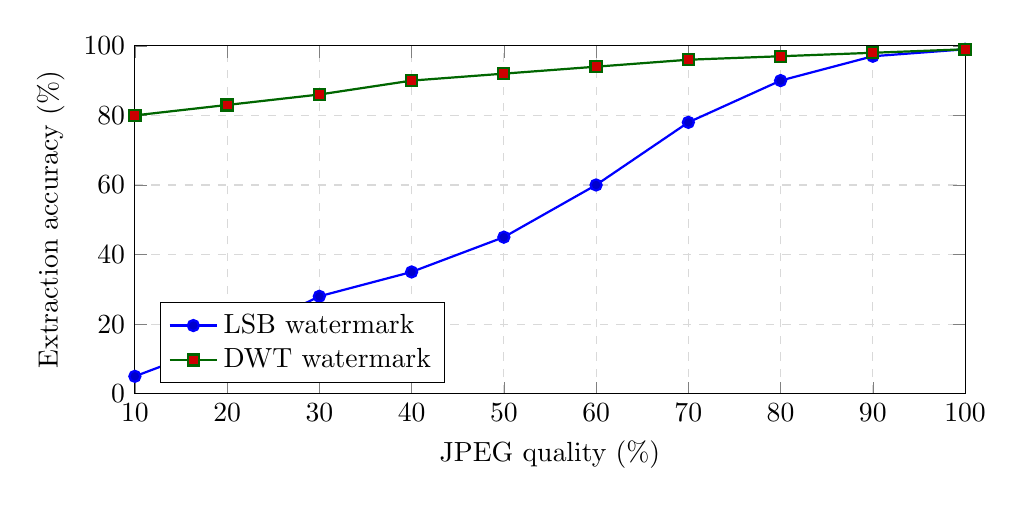
\begin{tikzpicture}
\begin{axis}[
    width=\linewidth,
    height=6cm,
    xlabel={JPEG quality (\%)},
    ylabel={Extraction accuracy (\%)},
    ymin=0,ymax=100,
    xmax=100,xmin=10,
    legend pos=south west,
    legend cell align=left,
    ymajorgrids,
    xmajorgrids,
    grid style={dashed,gray!30},
]
\addplot+[thick,blue,mark=*] coordinates {
  (10,5) (20,15) (30,28) (40,35) (50,45) (60,60) (70,78) (80,90) (90,97) (100,99)
};
\addlegendentry{LSB watermark}

\addplot+[thick,black!60!green,mark=square*] coordinates {
  (10,80) (20,83) (30,86) (40,90) (50,92) (60,94) (70,96) (80,97) (90,98) (100,99)
};
\addlegendentry{DWT watermark}
\end{axis}
\end{tikzpicture}

\caption{Extraction accuracy vs JPEG quality (representative).}\label{fig:app:robustness_curve}
\end{figure}

\section*{Latency Distribution}
\begin{figure}[ht]
  \centering
  % # TODO: Generated plot; run `make analyze` to produce toolset/figures/anchoring_cost_generated.tikz.tex
  \input{toolset/figures/anchoring_cost_generated.tikz.tex}\caption{Latency / anchoring cost breakdown (auto-generated).}\label{fig:app:anchoring_cost}
\end{figure}

\section*{Summary Table}
% # TODO: Generated table; run `make analyze` to produce results/figures/latency_table_generated.tex
\IfFileExists{results/figures/latency_table_generated.tex}{\input{results/figures/latency_table_generated}}{(Latency table not yet generated.)}

\paragraph{Reproduction.} Invoke:
\begin{minted}[fontsize=\scriptsize]{bash}
make analyze   # regenerates metrics + figures
make build     # embeds refreshed assets
\end{minted}

All plot inputs reside under \texttt{toolset/} and \texttt{results/} subtrees; git
history tracks provenance hashes for audit.
